\chapter{\acl{SUSY}}
\label{sec:susy}
The \ac{SM}, as described in Chapter~\ref{sec:sm} appears to describe all the
known fundamental particles and interactions to an incredible degree of
accuracy. What cause is there to believe that there might be physical phenomena
not described by this theory? This will be the topic we now turn to.

\section{Limitations of the \acl{SM}}
\label{sec:susy_limitations_sm}
A limitation immediately apparent in the \ac{SM} is that it makes no attempt to
unify gravity with the other fundamental forces. From a purely experimental
perspective, this is not an issues, since no experiment is able to explore
gravitational effects at the quantum scale. This is not likely to change in the
foreseeable future. However, it seems certain to many theorists that a quantised
theory of gravity must exist and indeed this has been the focus of great
theoretical effort in the last thirty years. Several potential theories have
emerged, aiming to provide an entirely unified picture of fundamental physics;
two examples being \emph{string theory} and \emph{loop quantum gravity}. Whilst
proponents of these theories have been criticised for devising untestable
hypotheses, it ``feel right'' to many physicists that new physics must be
present to give a more unified physical theory.

\subsection{The Hierarchy Problem}
The \emph{hierarchy problem} is arguably one of the strongest theoretical
arguments for physics beyond the \ac{SM}. This relates to the apparently huge
difference between the weak mass scale (\Mweak) and the Planck scale of gravity
(\Mplanck) - over 16 orders of magnitude. To some, it seems unthinkable that no
new physics should appear in this vast range of energies.

As well as being aesthetically undesirable, the hierarchy problem presents a
real theoretical issue for the mass of the Higgs boson. The Higgs boson mass
receives quantum corrections from every particle that it couples to - directly
or indirectly. These corrections have the form,
\begin{equation}
\Delta \mHiggs^2 = -\frac{\left|\lambda_f\right|^2}{8\pi^2}\LambdaUV^2 + \ldots
\label{eqn:higgs_mass}
\end{equation}
where $\lambda_f$ is a coupling constant to a fermion $f$ and \LambdaUV is the
momentum cut-off regulating the loop integral. All \ac{SM} fermions can
contribute to this correction, which is largest for the top quark with
$\lambda_f \approx 1$. Interpreting $\LambdaUV$ as the scale at which new
physics should appear to alter the behaviour of the theory and taking this to be
the Planck scale, these corrections are found to be 30 orders of magnitude
larger than the expected Higgs mass ($\approx \unit{100}{\GeV}$).

Whilst it might seem possible to just pick a small value of \LambdaUV, this
would require some form of new physics at this scale to alter the propagators in
the loop as well as cutting off the loop integral. As will be seen \ac{SUSY}
provides a neat solution to this problem.

\subsection{Dark Matter}
\label{sec:susy_darkmatter}
The problem of Dark Matter is perhaps the most convincing argument, at least to
experimentalists for the existence of some physics beyond the \ac{SM}. It was
observed as early as 1932 \cite{darkmatter_review} that galactic rotation curves
appeared to be at odds with those predicted from an estimation of their visible
mass. This seems to suggest a great deal of additional mass is present in the
galaxy, over and above that which can be inferred from the visible matter. This
observation is confirmed by measurements of gravitational lensing
\cite{bullet_cluster} and mapping of the cosmic microwave background
\cite{wmap_7year}. Current observations suggest dark matter comprises more than
80\% (TODO:citation needed) of the matter content of the universe. No
experimentally confirmed theory is able to match such a prediction.

Because of its invisible nature, a possible explanation for Dark Matter is a
\acl{WIMP}. Experiment hoping to directly detect such a particle have been
underway for some time. Typically, a large volume of a suitable gas or liquid is
used in the hope that passing \acp{WIMP} will undergo a nuclear
interaction. Whilst discoveries have been claimed, the evidence is not yet
believe to be conclusive \cite{dama_libra}.

A related issue is that of Dark Energy - believed to constitute nearly
three-quarters of the mass-energy content of the universe. This is an effect not
predicted by the currently accepted theories of particle physics. Taken
together, these phenomena are strong evidence of physics beyond the \ac{SM}.

\section{Beyond the \acl{SM}}
Having provided some motivation for looking beyond the \ac{SM} towards a more
complete theory, the question is then what sort of new physics might be
expected. The success of the \ac{SM} suggested an immediate path to predicting
new physics - namely extending the gauge group
$\SUthree_C\times\SUtwo_L\times\Uone$ to include an additional symmetry. There
are several ways one might imagine doing this\footnote{This list is not intended
  to be exhaustive but only to highlight a few popular approaches to the problem}:
\begin{itemize}
\item or a shift beyond gauge theories to a new theoretical paradigm.
\item extending the \ac{SM} gauge group with an additional symmetry or embedding
  the symmetry within a larger group;
\item proposing some new theory which extends the symmetry group of spacetime -
  the \Poincare group;
\end{itemize}

Examples of the first approach have already been mentioned - string theory, loop
quantum gravity and numerous others. Nothing further will be said of these
except that, whilst not making predictions testable by contemporary experiments,
they do in certain cases suggest extensions of the \ac{SM} which might fit under
the second and third bullet points (for instance in the case of supersymmetry).

Many attempts have been made to construct a \acl{GUT} using the first
approach. The Georgi-Glashow model \cite{georgi_glashow}, for instance, embeds
the \ac{SM} into the \SUfive group. This suffers from a number of problems - in
particular predicting unstable protons - but is otherwise quite successful as a
description of the \ac{SM}.

Finally, the last kind of extension has also attracted considerable theoretical
interest. Much of this was forever stymied by a so-called ``no go theorem''
published by Coleman and Mandula in 1967 \cite{coleman_mandula}. This
essentially forbids a class of extensions to the \ac{SM} which attempt to
combine the \Poincare group with an additional symmetry beyond just as a simple
product. Put precisely \cite{sparticles}, the Lie algebra representing the
continuous symmetries of the S matrix, containing as subalgebras the \Poincare
Lie algebra and some other Lie algebra defined by generators $T^a$ and structure
constants $t^{ab}_c$ must be a direct sum of the two algebras i.e.
\begin{equation}
\left[T^a, P_{\mu}\right] = \left[T^a, M_{\mu\nu}\right] = 0
\end{equation}
where $P_{\mu}$ and $M_{\mu\nu}$ are generators representing translations and
rotations/boosts in the \Poincare group. Commutativity of the generators implies
that the group may be separated into a simple product of two groups.

However, it turns out the technical requirements of this theorem, namely that it
applies exclusively to Lie algebras, points to a potential escape route. As will
be seen, this limitation allows \acl{SUSY} to neatly sidestep the
Coleman-Mandula theorem and introduce an additional, non-trivial space-time
symmetry. The next section will explain how this is done and, importantly how it
solves the issues introduced in Section~\ref{sec:susy_limitations_sm}.

\section{\acl{SUSY}}
\subsection{An Additional Symmetry}
The central concept of \ac{SUSY} is to impose an additional spacetime symmetry:
a symmetry between bosons and fermions. Whilst at first this might seem to fall
foul of the Coleman-Mandula theorem, it can be seen that this additional
``supersymmetry'' must be an anti-commuting spinor \Qa (where the subscript $a$
is a spinor index). As for other spinors, this has an anti-spinor, \AQa. The
algebra representing this transformation is no longer a Lie Algebra, which
requires commutation relations, but a ``Lie superalgebra'' obeying
\emph{anti-commutation} relations.

Supersymmetric theories are therefore not subject to the Coleman-Mandula
theorem, but instead to the Haag, Lopuszanski, Sohnius theorem. This will not be
stated explicitly but it places restrictions on the form of the \ac{SUSY}
algebra. These have the schematic form \cite{susy_primer}:
\begin{eqnarray}
\left\{Q,Q^{\dagger}\right\} = P^{\mu}\\
\left\{Q,Q\right\} = \left\{Q^{\dagger}, Q^{\dagger}\right\} = 0\\
\left[P^{\mu}, Q\right] = \left[P^{\mu}, Q^{\dagger}\right] = 0\label{eqn:susy_commutator}
\end{eqnarray}
where spinor indices have been dropped.

\subsection{Consequences}
\label{sec:consequences}
This seemingly simple addition brings with it a very rich phenomenology. Most
importantly, from the point of view of experimental physics, it predicts a large
number of new particles. Each particle in a supersymmetric theory is paired with
another in a so-called ``supermultiplet''. These particles are said to be
``superpartners'' of one another and are related by a supersymmetry
transformation.

It can be shown (see \cite{susy_primer}) that each supermultiplet should contain
an equal number of bosonic and fermionic degrees of freedom. This allows the
range of possible supermultiplets to be enumerated. The simplest such
possibility must contain a spinor with two fermionic degrees of freedom. This
implies that it should also contain two bosonic degrees of freedom: either as
two real scalar fields or a single complex scalar field. This pairing is known
as a \emph{chiral supermultiplet}.

Imagining next a supermultiplet containing a massless spin 1 boson (these have
two helicity states, and thus two bosonic degrees of freedom). This must be
paired with a single massless spinor with two fermionic degrees of freedom. This
must have \spinhalf (a \spinthreetwo particle would would cause renormalisation
problems). This pairing is known as a \emph{vector supermultiplet}.

Supersymmetry therefore requires the placing of all \ac{SM} particles into one
of these supermultiplets. Inevitably, this would require the existence of a
whole range of additional particles - each possessing a spin differing by
$\frac{1}{2}$ from its \ac{SM} counterpart.

In addition to having a certain theoretical elegance, this turns out to address
the major problems pointed out in
Section~\ref{sec:susy_limitations_sm}. Firstly, it provides a remedy to the
hierarchy problem. The additional superpartners also contribute to the Higgs
mass corrections (see Equation~\ref{eqn:higgs_mass}). In fact, bosonic and
fermionic loops contributing to the correction, appear with opposite
signs. \acl{SUSY} therefore causes exact cancellations of these problematic
contributions - effectively solving the hierarchy problem.

A certain class of supersymmetric theories also contain a solution to the Dark
Matter puzzle. Such theories contain a \acl{LSP} which appears to match the
characteristics of a \ac{WIMP}.

Finally, another aspect of \ac{SUSY} theories that is often touted as an
advantage is that it allows the gauge couplings for the electromagnetic, weak
and strong forces to unify at a certain energy scale. The running of the inverse
couplings is shown in Figure~\ref{fig:susy_gauge_unification}.

\subsection[R-Parity]{\Rparity}
When it comes to writing down a supersymmetric Lagrangian, it is possible to
write down terms which violate either Baryon ($B$) or Lepton number ($L$)
conservation. Such terms are forbidden in the \ac{SM} by renormalisability
requirements. Such $B$ or $L$ violation would imply proton decay times much
shorter than experimental lower limits. In order to prevent such terms from
appearing in the Lagrangian, a new discrete symmetry is supposed, \Rparity.

\Rparity is often considered as a new quantum number possessed by each particle
and multiplicatively conserved,
\begin{equation}
\PR = \left(-1\right)^{3(B-L)+2s}
\end{equation}
where $s$ is the spin of the particle. This results in an assignment of $\PR =
1$ to all \ac{SM} particles, and -1 to their superpartners. \ac{SUSY} particles
may only be produced from \ac{SM} particles in pairs and their decays must also
result in an odd number of \ac{SUSY} particles.

The importance of this becomes clear when one considers the lightest
superpartner in the theory (the aforementioned \ac{LSP}). This is unable to
decay to a lighter \ac{SUSY} particle and thus is unable to satisfy the
requirements of \Rparity conservation. It is therefore stable and, under certain
other assumptions, a suitable candidate for the \ac{WIMP} hypothesised to solve
the Dark Mater problem.

\begin{figure}
\centering
\includegraphics[width=0.7\textwidth]{fig/unification}
\caption{Two-loop renormalisation group evolution of the inverse gauge couplings
  $\alpha_a^{−1}(Q)$ in the \ac{SM} (dashed lines) and the MSSM (solid
  lines). In the MSSM case, the sparticle masses are treated as a common
  threshold varied between \unit{500}{\GeV} and \unit{1.5}{\TeV}, and
  $\alpha_3(mZ)$ is varied between $0.117$ and $0.121$. \cite{susy_primer}}
\label{fig:susy_gauge_unification}
\end{figure}

\subsection{\ac{SUSY} Breaking}
Things are never quite so simple unfortunately. Examining the commutator in
Eqn~\ref{eqn:susy_commutator}, it is seen that the \ac{SUSY} generator \Qa
commutes with $P^{\mu}$ and hence also $P^{\mu}P_{\mu} = m^2$. The consequence
of this is that superpartners should have equal mass. This is clearly at odd
with experiment, since no additional superpartners have so far been
observed.

If supersymmetry is to be a symmetry of the universe, some additional mechanism
must be incorporated into the theory to explain these differing masses. Taking
inspiration from \ac{EWSB}, the supersymmetry is said to be spontaneously
broken. Supersymmetry would therefore be respected by the Lagrangian but not by
the vacuum. This would effectively ``hide'' supersymmetry at lower mass scales
(i.e. those so far explored by experiment). There are several proposed
mechanisms for supersymmetry breaking. These will be discussed more fully at a
later point.

Throughout, discussion will be restricted to so-called ``soft'' \ac{SUSY}
breaking. Having invoked supersymmetry initially as a solution to the hierarchy
problem, it is desirable that the breaking of \ac{SUSY} not prevent the
cancellations which stabilise the Higgs mass. This restricts \ac{SUSY} breaking
terms in the Lagrangian to ones with positive mass dimension
\cite{susy_primer}. These is known as soft \ac{SUSY} breaking.


\section{\acl{MSSM}}
The \acl{MSSM} is a minimal extension of the \ac{SM} to include soft
\ac{SUSY}-breaking terms. Since the mechanism and dynamics of this breaking are
unknown, additional parameters must be introduced into the theory. The \ac{MSSM}
adds 105 additional real constants to the 19 present in the \ac{SM}. This proves
% See Sparticles pp 186
extraordinarily problematic from the point of view of experimental \ac{SUSY}
searches. In Chapter~\ref{sec:framework}, it will be shown how simplified models
can offer a much simpler context for interpretation of results.

\subsection{Particle Content}
We shall now discuss the particle content of the \ac{MSSM}, a summary of which
is presented in Tables~\ref{tbl:susy_particles} and \ref{tbl:susy_gauginos}. The
basic forms of allowed supermultiplets were discussed in
Section~\ref{sec:consequences}. Each fermion in the \ac{SM} is placed into a
chiral supermultiplet with a \spinzero ``sfermion''. These are written with a
tilde, e.g. $\PSe_L$ for the ``selectron''. Left-handed and right-handed
components must lie in separate chiral supermultiplets. It is important to note
that the subscripts on the sfermions indicate the chirality of the partner
fermion. Being \spinzero bosons, the sfermions are not chiral.

Similarly the \ac{SM} gauge bosons are placed into gauge supermultiplets. The
corresponding superpartners are referred to generically as ``gauginos'' or more
specifically as ``Winos'', ``Bino'', ``gluinos''. Electroweak symmetry breaking
(see Section~\ref{sec:theory_ewsb}) leads to the mixing of the gauge eigenstates
$\PW^0$ and $\PB^0$ to give $\PZ$ and $\Pphoton$. The corresponding combinations
of superpartners are known as the Zino (\PSZ) and Photino ($\PSphotino$)
respectively.

For the Higgs field, one might expect it to be placed into a single chiral
supermultiplet with a \spinhalf superpartner. This turns out not to be possible
for two reasons. Firstly, for reasons beyond the scope of this discussion, such
a theory would suffer a gauge anomaly after quantisation. Secondly, the
structure of the Yukawa couplings (see Section~\ref{sec:theory_yukawa}) actually
requires two Higgs supermultiplets to give mass to up and down type quarks. The
complex scalar doublets with hypercharge, $Y=\pm\frac{1}{2}$ will be referred to
as $\PHiggs_u$ and $\PHiggs_d$ respectively. The weak isospin components of
these are then $\PHiggs_u^+$, $\PHiggs_u^0$, $\PHiggs_d^0$ and $\PHiggs_d^-$
where the superscript indicates electric charge.

The fermionic superpartners of each Higgs field, the Higgsinos, are then denoted
$\PSHiggs_u$ and $\PSHiggs_d$. The physical \ac{SM} Higgs is taken to be a
linear combination of the neutral components $\PHiggs_u^0$ and $\PHiggs_d^0$.

\ctable[
cap=Chiral supermultiplets in the \acs{MSSM},
caption=Chiral supermultiplets in the
\acs{MSSM}~\cite{susy_primer}. Right-handed neutrino fields and their
corresponding superpartners are not shown.,
label=tbl:susy_particles,
pos=h
]{cccc}{
}{\FL
\multicolumn{2}{c}{\spinzero} & \multicolumn{2}{c}{\spinhalf} \ML
Squarks & $\tilde{Q} = \left(\begin{array}{c} \PSup_{\textrm{L}} \\ \PSdown_{\textrm{L}}\end{array}\right)$ & Quarks & $Q = \left(\begin{array}{c} \Pup_{\textrm{L}} \\ \Pdown_{\textrm{L}}\end{array}\right)$\NN
 & $\PSup_{\textrm{R}}$ & & $\Pup_{\textrm{R}}$\NN
 & $\PSdown_{\textrm{R}}$ & & $\Pdown_{\textrm{R}}$\ML
Sleptons & $\tilde{L} = \left(\begin{array}{c} \PSnu_{\textrm{L}} \\ \PSlepton_{\textrm{L}}\end{array}\right)$ & Leptons & $L = \left(\begin{array}{c} \Pneutrino_{\textrm{L}} \\ \Plepton_{\textrm{L}}\end{array}\right)$\NN
 & $\PSlepton_{\textrm{R}}$ & & $\Plepton_{\textrm{R}}$\ML
Higgs & $\PHiggs_u = \left(\begin{array}{c} \PHiggs^+_{u} \\ \PHiggs^0_{u}\end{array}\right)$ & Higgsinos & $\PSHiggs_u = \left(\begin{array}{c} \PSHiggs^+_u \\ \PSHiggs^0_u\end{array}\right)$\NN
 & $\PHiggs_d = \left(\begin{array}{c} \PHiggs^0_{d} \\ \PHiggs^-_{d}\end{array}\right)$ &  & $\PSHiggs_d = \left(\begin{array}{c} \PSHiggs^0_d \\ \PSHiggs^-_d\end{array}\right)$\LL
}

\ctable[
caption=Gauginos,
mincapwidth=0.75\textwidth,
label=tbl:susy_gauginos,
pos=h
]{cccc}{
}{\FL
\multicolumn{2}{c}{\spinhalf} & \multicolumn{2}{c}{\spinone} \ML
Gluino & \PSgluino & Gluon & \Pgluon \NN
Winos  & $\PSWino^0$, \PSWpm   & Weak bosons & \PWpm, $\PW^0$\NN
Binos  & $\PSBino^0$           & B boson     & \PB\LL
}


\subsection{Neutralinos and Charginos}
Electroweak symmetry breaking leads to mixing of the charged and neutral gaugino
eigenstates. The four mass eigenstates formed from the charged gauginos are
known as \emph{charginos}. They are composed of the charged Higgsinos
($\PSHiggs_u^+$, $\PSHiggs_d^-$) and Winos ($\PSWpm$). The four chargino states
are therefore $\PScharginopm_i$ for $i=1,2$. Similarly the neutral Higgsinos
($\PSHiggs_u^0$, $\PSHiggs_d^0$), Wino ($\PSW^0$) and Binos ($\PSB^0$) mix to
give four \emph{neutralinos}. These will be denoted $\PSneutralino_i$ where
$i=1,2,3,4$. The lightest of these will be denoted \PSneutralino. This is often
taken to be the dark matter candidate referred to in
Section~\ref{sec:consequences}.

\section{Supersymmetry Searches}
Since the emergence of supersymmetry in the 1970s, a number of particle physics
experiments have undertaken dedicated searches for evidence of supersymmetric
particles. These collider or fixed-target experiments have sought to produce
supersymmetric particles in high-energy collisions - so far without success
\cite{ua1_susy, aleph_susy, d0_susy, hera_susy}. As discussed in
Section~\ref{sec:susy_darkmatter}, dedicated searches have also been performed
specifically for ``\ac{WIMP}-like'' Dark Matter signals. The detection
experiments will not be discussed further here, except to say that they offer a
highly complementary path to the discovery of Dark Matter
\cite{mastercode_2011}.

In this section, the constraints set by previous supersymmetry searches will be
summarised. This will naturally motivate discussion of the experimental
signatures of \ac{SUSY} particles. Finally, the signatures most relevant for
searches at the \ac{LHC} will be presented, in particular the single lepton
channel that is the basis for the search described in
Chapter~\ref{sec:susysearch}.

\subsection{Superysymmetry at Colliders}
Useful experimental signatures of supersymmetry at colliders depend greatly on
whether \Rparity is assumed as a conserved quantity. Since, conservation of
\Rparity predicts the existence of a \ac{WIMP} particle and ensures a stable
proton, it is often assumed by experimental searches. \Rparity violating
theories are the subject of theoretical \cite{aulakh_rpv} and experimental work
but will not be discussed further here.

As stated previously, \Rparity conservation predicts the existence of a stable
\ac{LSP} or \ac{WIMP}. Being weakly interacting, this will not be directly
detected at a collider experiment but is observable as a deficit of energy in
the detector - a so-called missing energy signature. This signal forms the basis
of the vast majority of collider supersymmetry searches. In addition to one or
more \acp{LSP}, \ac{SUSY} decays typically result in a large number of \ac{SM}
particles. More will be said of this at a later point.
%TODO SUSY Higgs search

Whilst missing energy offers a relatively clean signature, \ac{SM} backgrounds
with a missing energy component may be further rejected by making further
selection on the final state particles in an event. These backgrounds may
contain genuine missing energy signal - in the form of a \ac{SM} neutrino - or
be the result of detector mismeasurement - a ``fake'' signal. Additional
requirements often exploit other features of \ac{SUSY} particle
production. Suitable choices will depend on the dominant \ac{SUSY} production
processes and therefore on the nature of the colliding particles
e.g. $\Pelectron\APelectron$, $\Pproton\APproton$, $\Pproton\Pproton$. In other
cases, such additional requirements may focus sensitivity to a more specific
class of supersymmetric models.

\subsubsection{$\Pelectron\APelectron$ Colliders}
All sparticles (excluding the gluino) may be produced in tree-level processes at
$Pelectron\APelectron$ colliders\cite{susy_primer}. The \ac{LEP} experiment
which ran up to centre of mass energies of \unit{209}{\GeV} has excluded all
charged sparticles up to masses of approximately half this energy. If the mass
splitting between a given sparticle and the \ac{LSP} is assumed to be smaller,
the detection efficiency becomes worse and these limits become weaker.

Taking as an example the pair-production of charginos. The charginos
subsequently decay to the \ac{LSP} in association with either: four jets, two
jets and 1 lepton, or two leptons of opposite charge \cite{sparticles}. Searches
at \ac{LEP} set a limit of $m_{\PScharginopm} > \unit{103}{\GeV}$ (or weaker if
the $\unit{100}{\MeV} m_{\PScharginopm} - m_{\PSneutralinoOne} < \unit{3}{\GeV}$
\cite{susy_primer}).

\subsubsection{Hadron Colliders}
At hadron colliders, production of charginos, neutralinos, sleptons and
sneutrinos is possible via electroweak processes. In addition, production of
squarks and gluinos is possible with \ac{QCD} strength. At Fermilab's Tevatron
accelerator, chargino and neutralino production normally dominate - unless the
squarks or gluinos are light. In contrast, at the \ac{LHC}, $\Psquark\Psquark$,
$\PSgluino\PSgluino$ or $\Psquark\PSgluino$ production are expected to dominate.

\Rparity requires that sparticles be pair produced. Each proceeds via a cascade
decay to the \ac{LSP}. The cascade will generally produce a number of jets and
possibly leptons. This covers most typical \ac{SUSY} topologies studied at
hadron colliders.

One such cascade decay is shown in Figure~\ref{fig:susy_1lep_decay}. This would
be a typical cascade decay leading to a single lepton type signature. Whilst
being less inclusive than the pure jets + missing energy signature, the addition
of a single lepton serves to significantly suppress the background from \ac{QCD}
events. With the addition of further kinematic requirements, this channel is
sensitive to a range of \ac{SUSY} scenarios, as will be seen in
Chapter~\ref{sec:susysearch}.

\begin{figure}
\centering
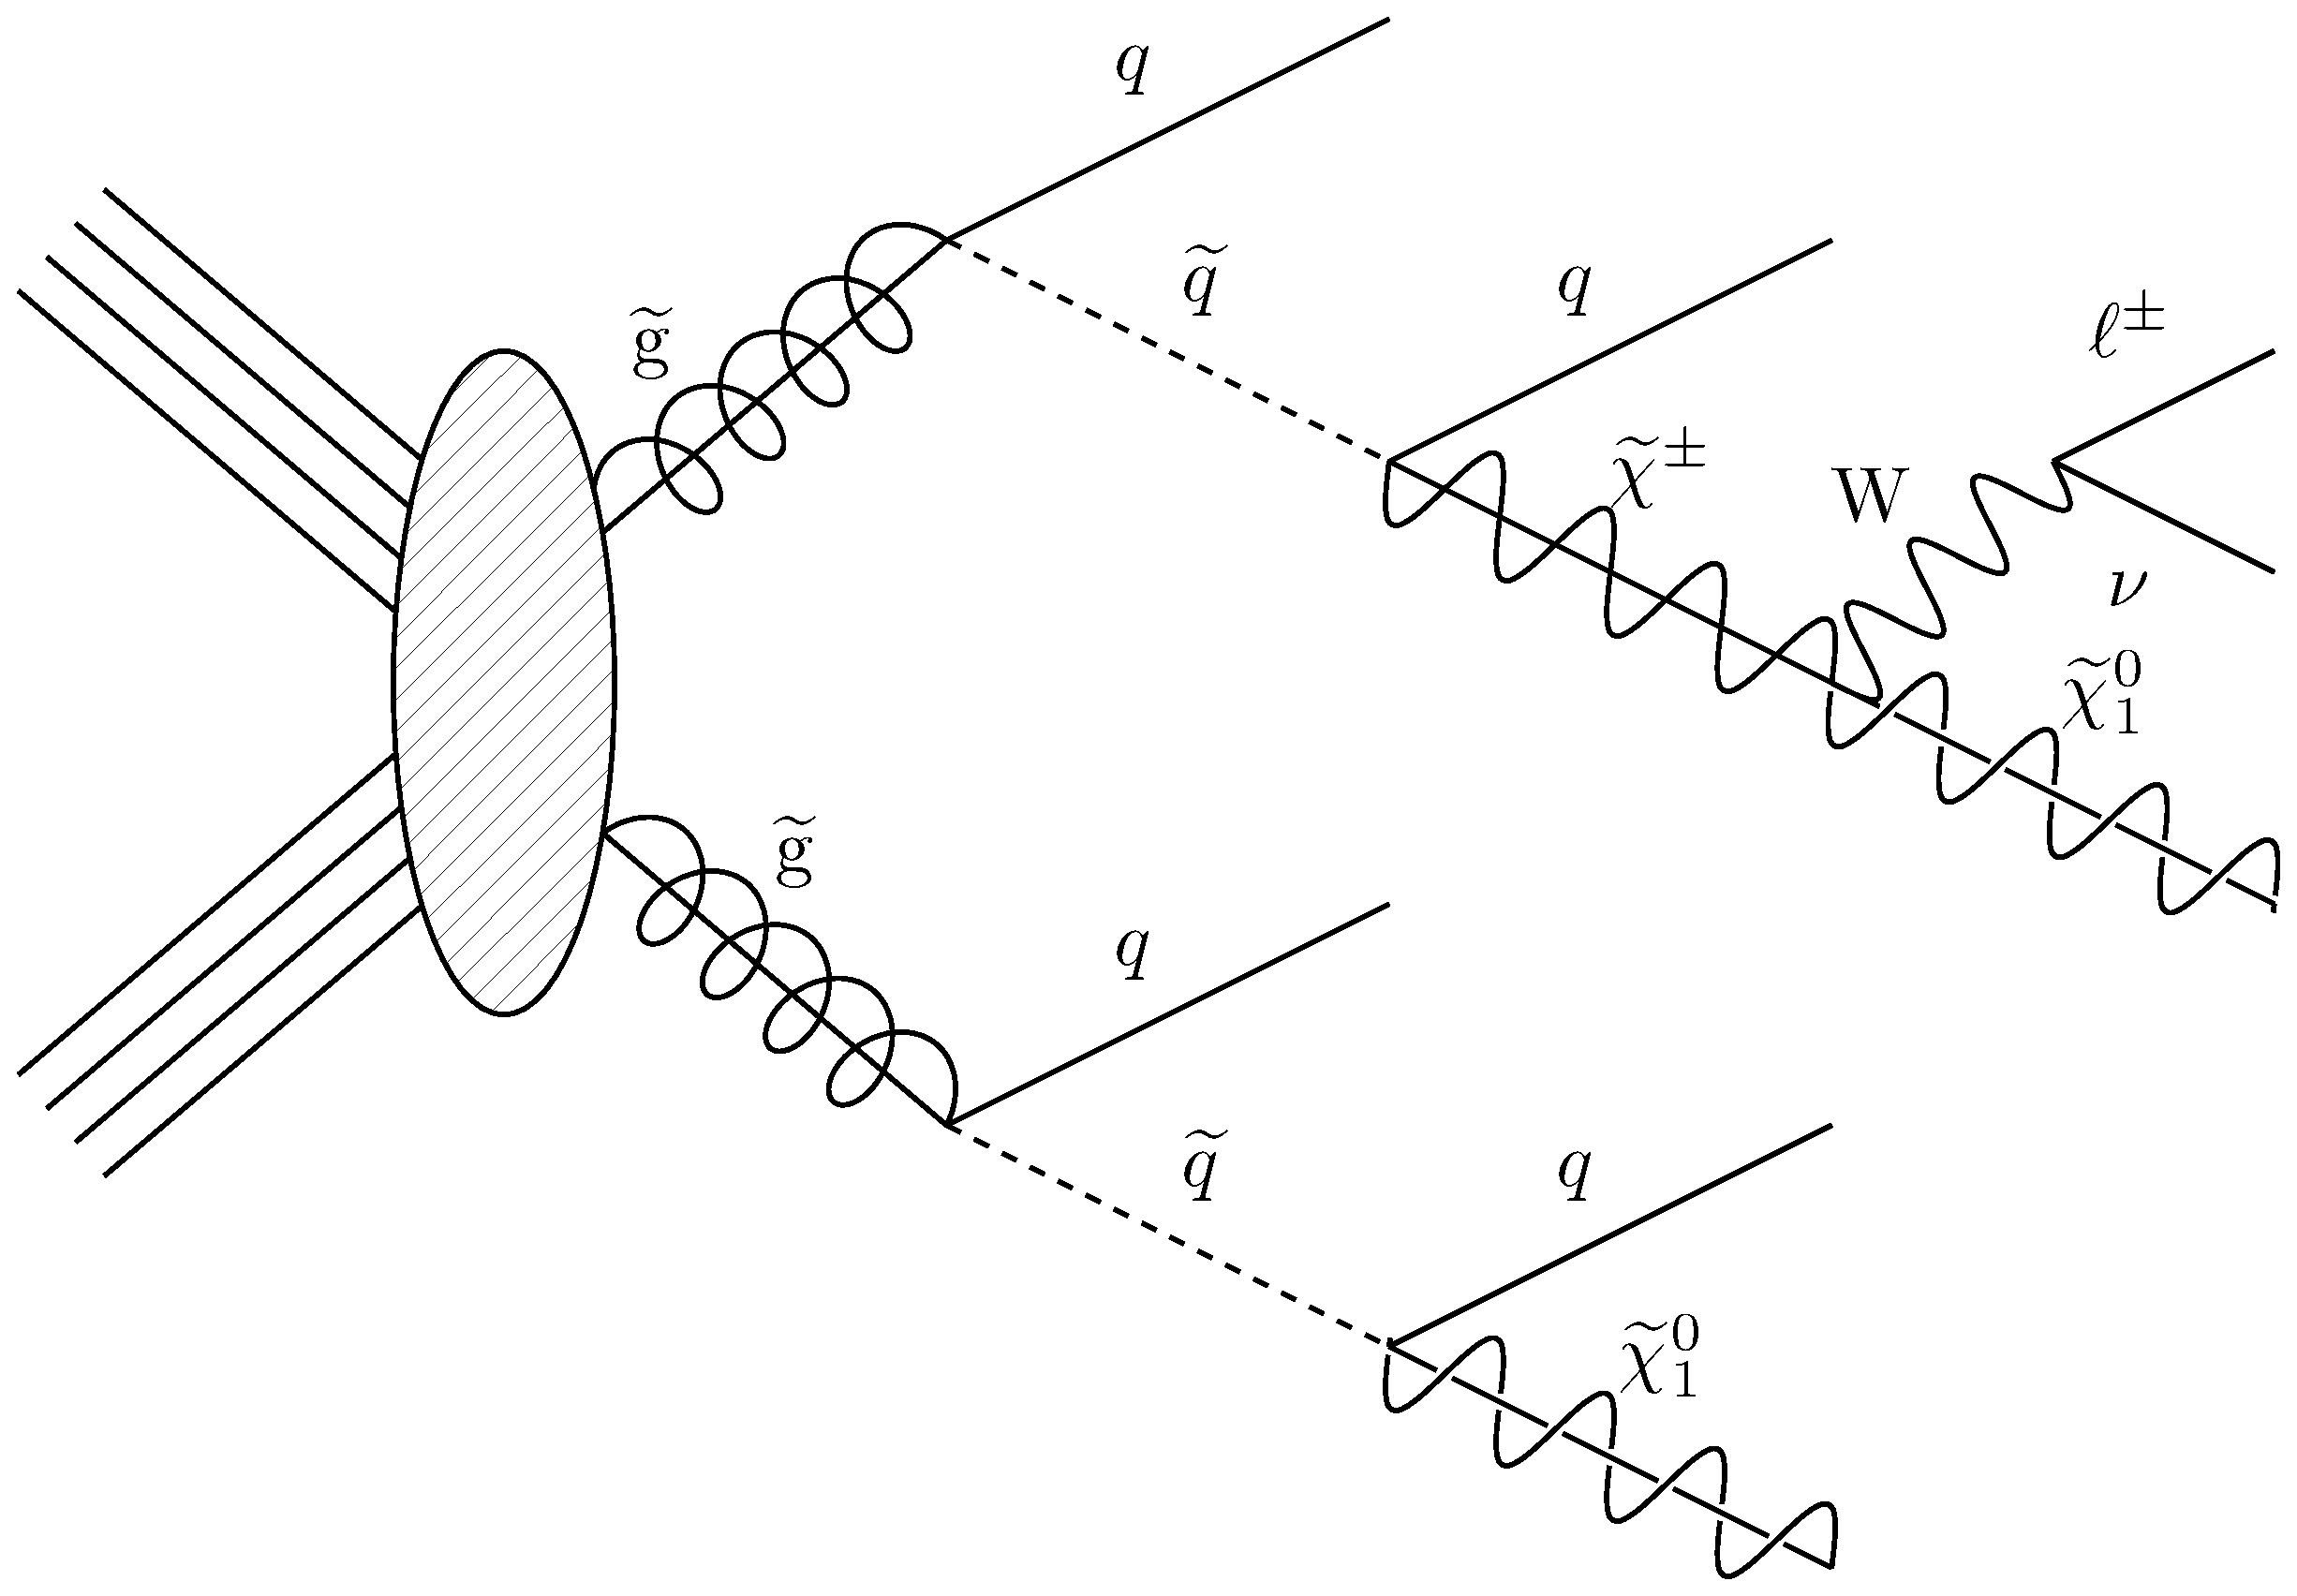
\includegraphics[width=0.7\textwidth]{fig/susy_1lep}
\caption{Diagram showing a possible \ac{SUSY} decay chain leading to a single lepton final state.}
\label{fig:susy_1lep_decay}
\end{figure}
